\documentclass[xcolor=dvipsnames,10pt]{beamer}

\beamersetaveragebackground{blue!10}

\mode<presentation>
{
     \usetheme{Warsaw}
}

\usepackage{polski}
\RequirePackage[utf8]{inputenc}

\author{Joanna Kotuła, Aleksandra Mogielska}
\institute[...]{Wydział Matematyki, Informatyki i Mechaniki\\
Uniwersytet Warszawski}

\subject{...}

\title[Intuicyjny język wyszukiwania TQL (Tablets Query Language)]{\bf  Intuicyjny język wyszukiwania TQL \\
Tablets Query Language}
%\subtitle{...}

\date{\today}



\begin{document}


\begin{frame}
     \titlepage
\end{frame}

%\begin{frame}
%     \frametitle{Spis treści}
%     \tableofcontents
%\end{frame}



\section{Domain Specific Languages}


\begin{frame}
     \frametitle{Domain Specific Languages (DSL)}
     
     DSL to języki przystosowane do używania w konkretnym celu.
     \begin{itemize}
          \item
          łatwość użycia
          \item
          specyficzne konstrukcje
          \item 
          ograniczone możliwości
          \item
          kompilacja do języka niższego poziomu (np. SQL)
     \end{itemize}


\end{frame}

\section{Tabliczki sumeryjskie}
%Coś o sumerach


\begin{frame}
     \frametitle{Tabliczki sumeryjskie}

\begin{columns}
\column{0.5\textwidth}
\begin{itemize}
\item gliniane tabliczki pokryte pismem klinowym
\item pochodzą z terenów Bliskiego Wschodu
\item najstarsze znane pismo (powstało ok. 3500r. p.n.e.)
%\item wiele zachowało się dzięki pożarom, ważniejsze wypalano specjalnie
%\item odciskane rylcem o trójkątnym przekroju
\item pismo początkowo rysunkowe, później coraz prostsze
\item głównie teksty gospodarcze i administracyjne% (dość regularne i rzeczowe)

\end{itemize}
\column{0.5\textwidth}
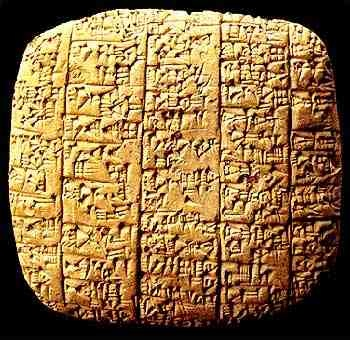
\includegraphics[width=55mm]{1/tablet.jpg}
\end{columns}
\end{frame}



\begin{frame}
\frametitle{Sumerologia}
    
\begin{columns}
 \column{0.5\textwidth}
Sumerologia to nauka badająca kulturę i historię starożytnych Sumerów, czerpiąca wiedzę m.in. z zachowanych tabliczek.
\begin{itemize}
\item zdigitalizowane i ręcznie skorygowane treści tabliczek są udostępnione przez system CDLI (obecnie prawie 225 000 tabliczek)
\item możliwość niewłaściwej interpretacji klinów
\item potrzebne intuicyjne narzędzie do wyszukiwania w bazie tabliczek na podstawie odczytów
\end{itemize} 

  \column{0.5\textwidth}
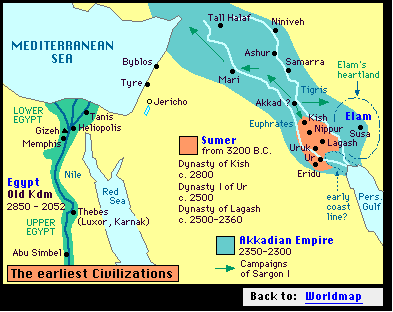
\includegraphics[width=55mm]{1/sum_map.png}
\end{columns}


\end{frame}


\section{Tablets Query Language}


\begin{frame}
     \frametitle{Tablets Query Language}
     \begin{itemize}
    \item Język pozwalający sumerologom łatwo tworzyć zapytania w bazie tabliczek.\\
   \item  Prosta składnia zapytań.\\
 \item    Zapytania zawierają informacje tylko o treści tabliczek i ich metadanych.\\
  \item   Możliwość stworzenia implementacji na dowolną bazę przechowującą tabliczki.\\ %ułatwiamy to dzięki podziałowi kodu na moduły

 \end{itemize}

\end{frame}
 
\begin{frame}

% dać składnię

     \frametitle{Przykładowe zapytania TQL}

\begin{block}{przykład 1}

provenience: Ur*\\
period: "Uruk III"\\
genre: Administrative\\
text: udu + (szid / sipa) $--$ adad-tilati\\

\end{block}
\end{frame}



\begin{frame}
\frametitle{Przykładowe zapytania TQL}
\begin{block}{przykład 2}
provenience: Gar*\\
period: UrIII\\
genre: Administrative\\
text: udu/masz2\\
~\\
provenience: Ur\\
period: UrIII\\
text: sig4\\
\end{block}
\end{frame}

\begin{frame}
 \frametitle{Przykładowe zapytania TQL}
\begin{block}{przykład 3}
define\\
  provenience: Garshana\\
  period: UrIII\\
  text: "udu ban"/mash2\\
as "zwierzaki w Garshana"\\
~\\
search\\
  text: adad-tilati\\
in "zwierzaki w Garshana"\\
\end{block}
\end{frame}


\section{Implementacja}
% Struktura translatora, opisać co się dzieje, dlaczego jest niezależne 
% itp., przepływ zapytania przez program
\begin{frame}
     \frametitle{Struktura}
\begin{center}
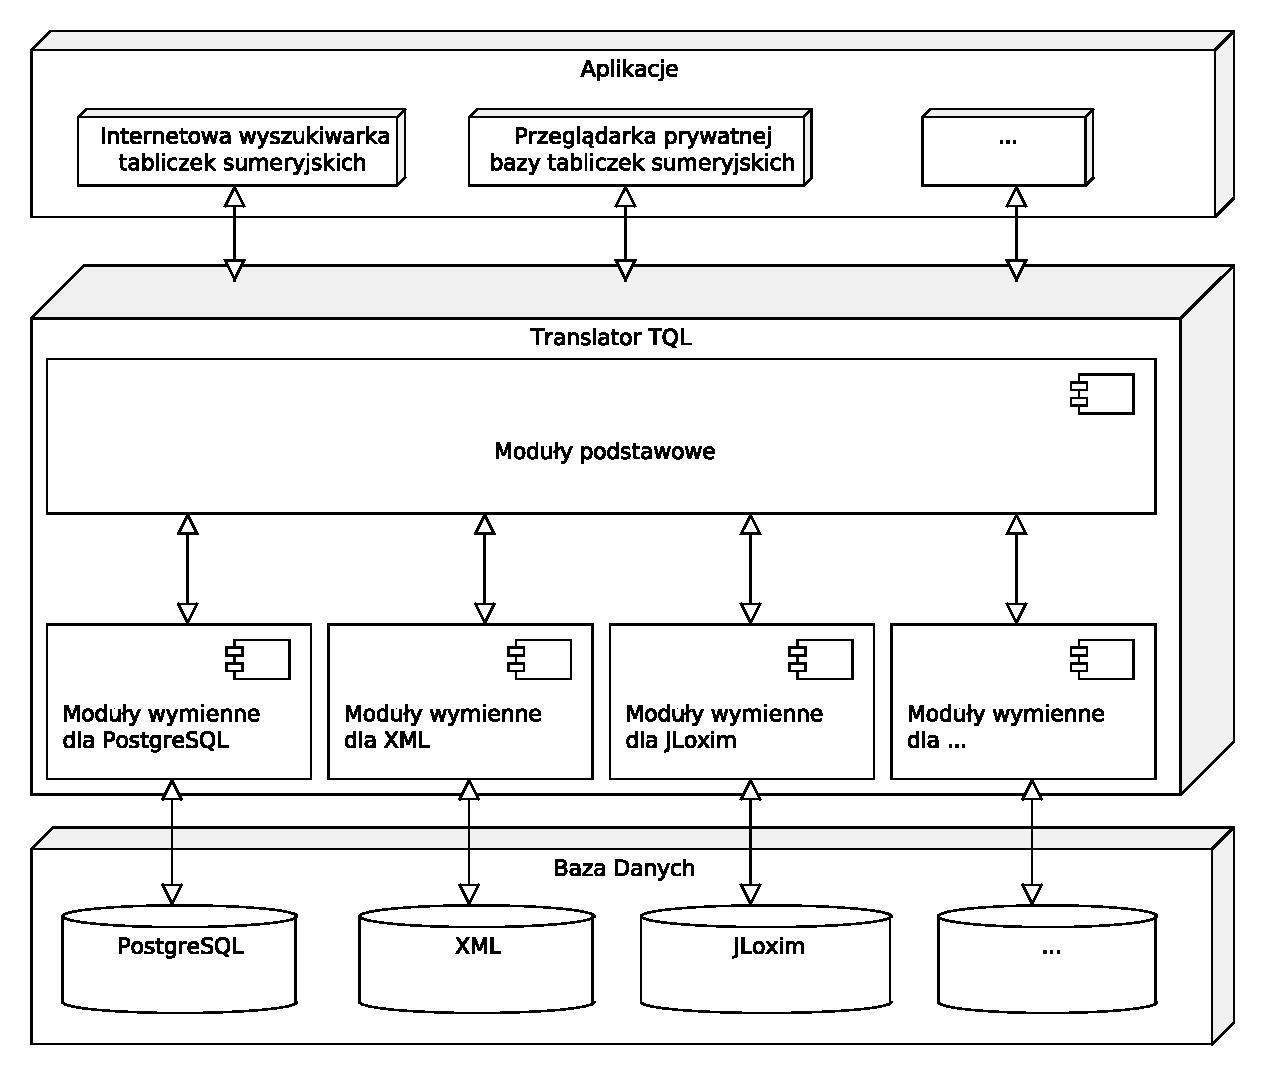
\includegraphics[height=70mm]{diagramy/struktura.pdf}
%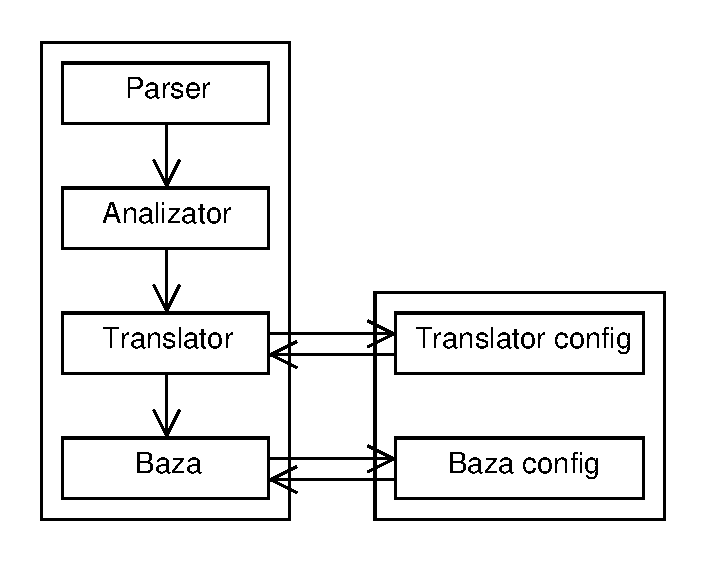
\includegraphics[height=70mm]{moduly.pdf}
\end{center}
\end{frame}


\begin{frame}
     \frametitle{Podział na moduły}
    
\begin{center}
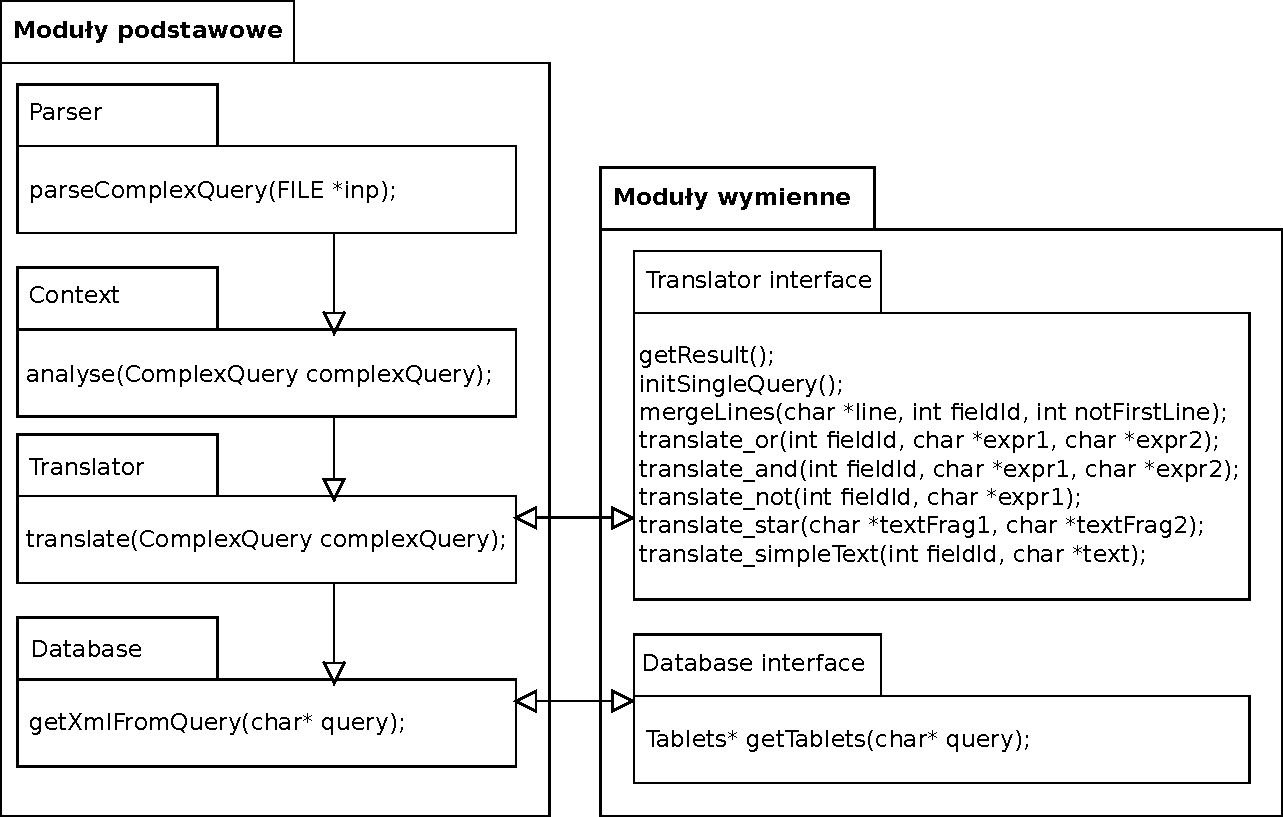
\includegraphics[width=100mm]{diagramy/pakiety.pdf}
%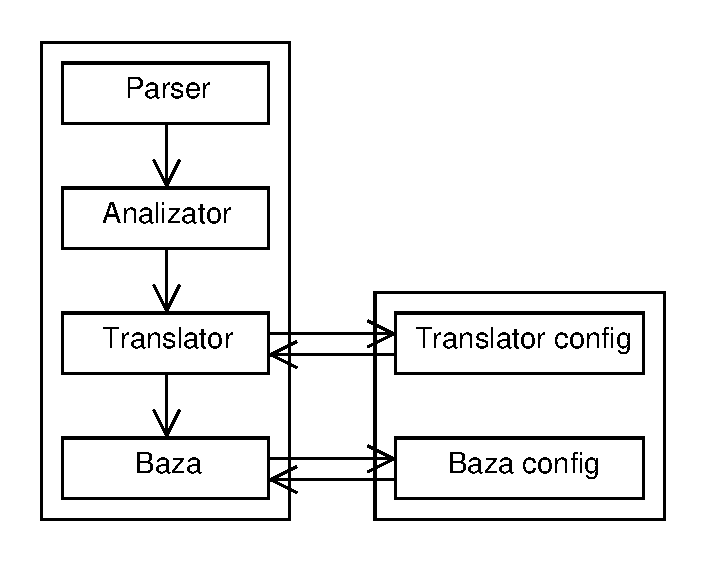
\includegraphics[height=70mm]{moduly.pdf}
\end{center}
\end{frame}

\begin{frame}
\frametitle{Parser i analizator składniowy}
\begin{itemize}
\item moduły niezależne od bazy danych i języka wyszukiwania
\item wspólne dla wszystkich  implementacji TQL
\item napisane za pomocą narzędzia BNFC, potem uporządkowane
\item wejście - zapytanie w języku TQL
\item wyjście - drzewo składni abstrakcyjnej
\end{itemize}
\end{frame}

\begin{frame}
\frametitle{Translator}
\begin{itemize}
\item wejście - drzewo składni abstrakcyjnej
\item wyjście - zapytanie w odpowiednim języku
\item buduje zapytanie:
\begin{itemize}
 \item przechodzi strukturę drzewa
 \item wywołuje funkcje z fragmentów zależnych od bazy danych (Translator\_interface.h)
 \item zwraca wynik (getResult())
\end{itemize}
\end{itemize}
\end{frame}


\begin{frame}
     \frametitle{Baza}
\begin{itemize}
\item wejście - zapytanie w języku docelowym
\item wyjście - XML zawierający informacje o znalezionych tabliczkach i ich treść
\item przekazuje zapytanie do części zależnej od bazy danych (Database\_interface.h)
\item dostaje strukturę
\end{itemize}
\end{frame}

\begin{frame}
 \frametitle{Baza}
\begin{columns}[t]
\column{.5\textwidth}
\begin{block}{Struktura Tablet}
typedef struct\{ \\
~~~~char* id; \\
~~~~char* id\_cdli; \\
~~~~char* publication; \\
~~~~char* measurements; \\
~~~~char* year; \\
~~~~char* provenience; \\
~~~~char* period; \\
~~~~char* genre; \\
~~~~char* subgenre; \\
~~~~char* collection; \\
~~~~char* text; \\
~~~~Tags *tags; \\
\} Tablet; \\
\end{block}
\column{.5\textwidth}
\begin{block}{Struktura Tablets}
typedef struct\{ \\
~~~~int size; \\
~~~~Tablet *tabs; \\
\} Tablets;
\end{block}
\end{columns}

\end{frame}

\subsection{PostgreSQL}
\begin{frame}
 \frametitle{Diagram encji}
 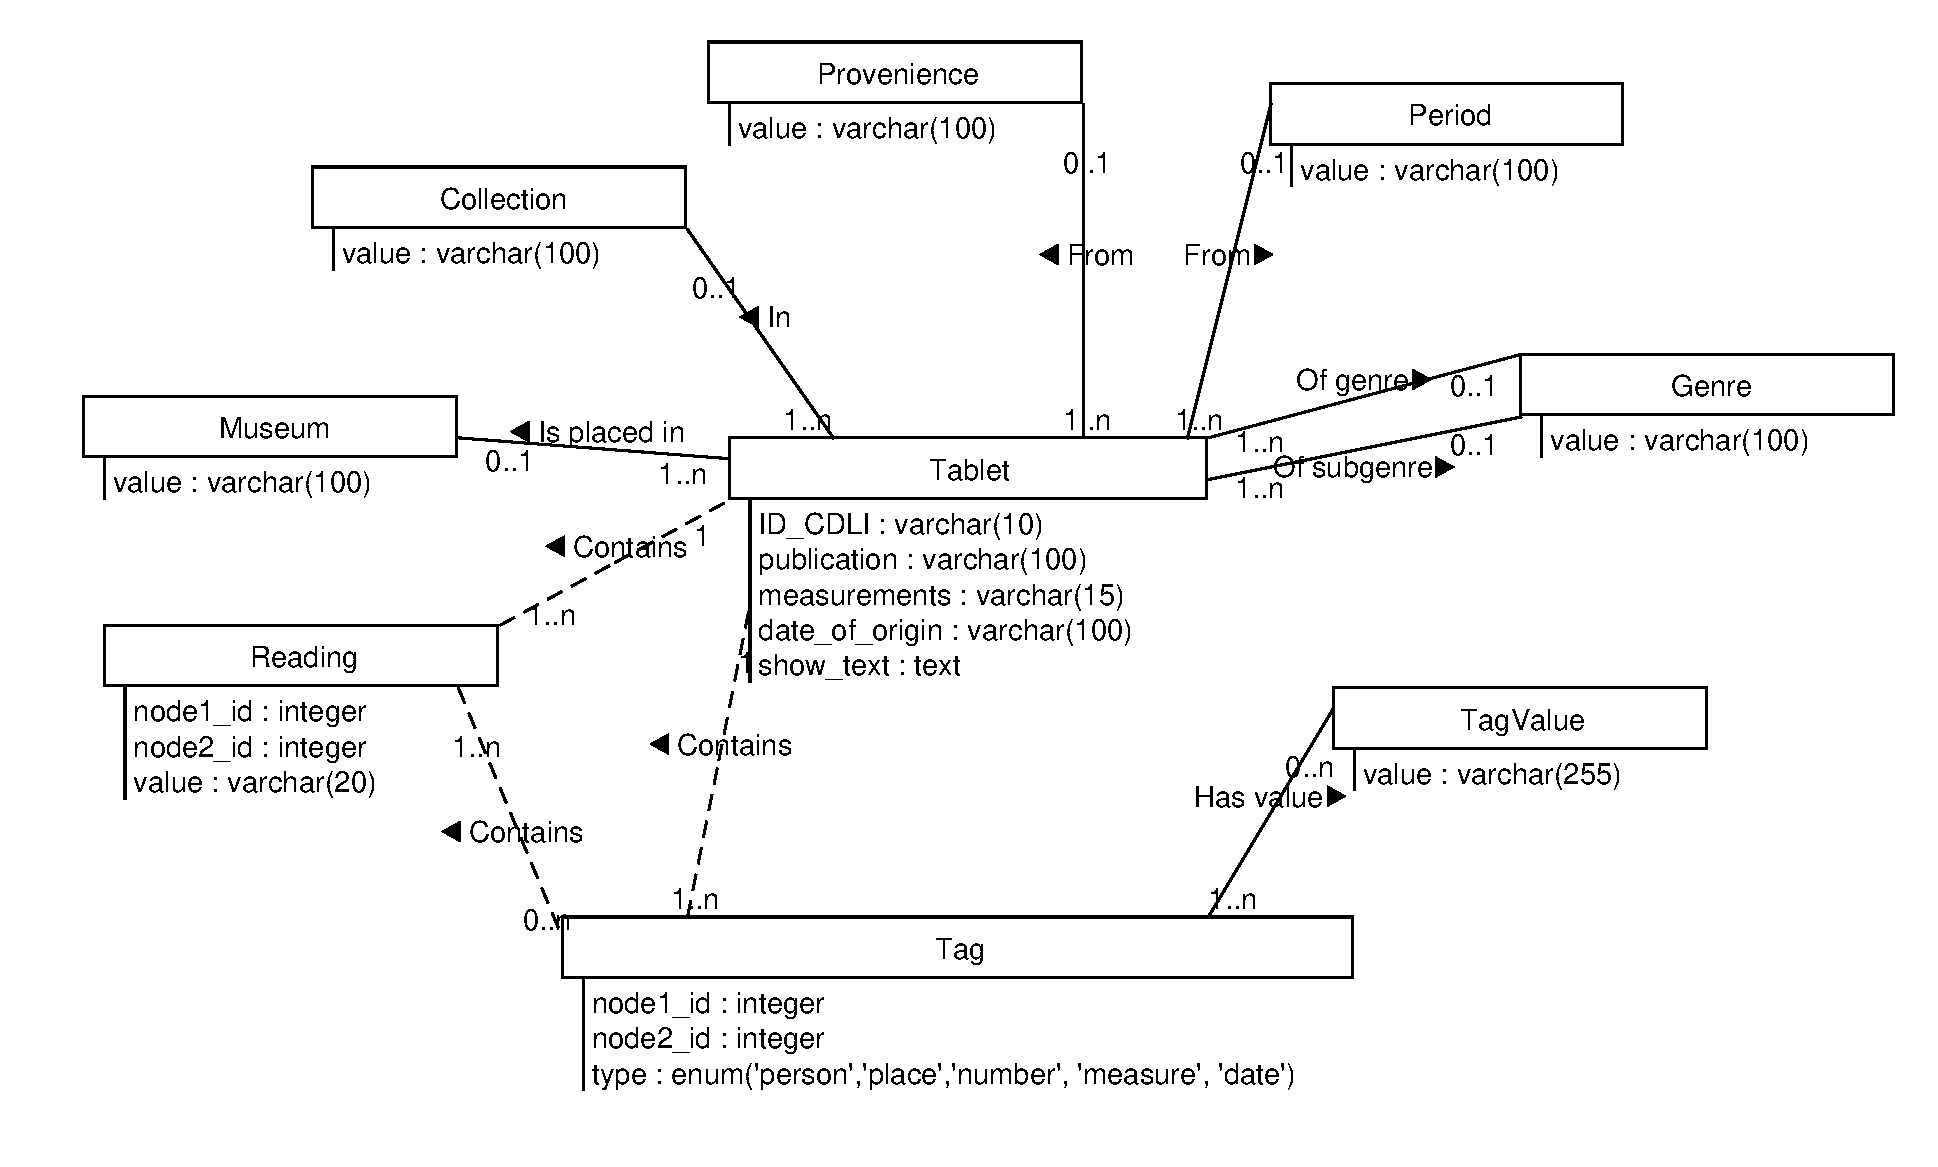
\includegraphics[width=100mm]{./diagramy/diagram-encji-maly.pdf}
\end{frame}


\subsection{XML}
\begin{frame}
 \frametitle{Schemat}

\end{frame}


% \begin{frame}
%      \frametitle{Aplikacja wykorzystująca translator}
%    
% \begin{itemize}
% \item umożliwa użytkownikowi wprowadzenie zapytania jako tekstu lub za pomocą graficznego interfejsu
% \item odpowiednio wyświetla zwracanego XML-a, pokazując wyszukiwane sekwencje
% \end{itemize}
% 
% \end{frame}
% 

% \section{Co zrobiłyśmy, co planujemy}
% %  Problemy (?) planowane optymalizacje (coś ciekawego na pewno musi 
% % być), featury (planowane)
% 
% 
% \begin{frame}
%      \frametitle{Do tej pory}
%      
% \begin{itemize}
% \item przykładowa baza relacyjna (Postgres)
% \item gotowy parser i analizator składniowy
% \item moduł translatora i moduł konfiguracyjny dla bazy relacyjnej
% \item moduł bazy: połączenie z bazą, wykonywanie zapytań i zwracanie XML-a -- jeszcze bez zaznaczonych sekwencji wyszukiwania
% \end{itemize}
% 
% 
% \end{frame}
% 
% \begin{frame}
%      \frametitle{Plany}
%      
% \begin{itemize}
% \item zaznaczanie w XML-u z tabliczkami wyszukiwanych sekwencji
% \item interfejs graficzny -- do wprowadzania zapytań i wyświetlania wyników
% \item moduły konfiguracyjne do innej bazy danych
% \item optymalizacje zapytań (obowiązkowo dla negacji)
% \item tłumaczenie odczyty $\leftrightarrow$  kliny i wyszukiwanie po klinach
% \end{itemize}
% \end{frame}
% 
%\section{Pokaz działania}

%\begin{frame}
%     \frametitle{Pokaz działania}
%\end{frame}


\end{document}




